\documentclass[letterpaper,11pt]{article}
\oddsidemargin -1.0cm \textwidth 17.5cm

\usepackage[utf8]{inputenc}
\usepackage[activeacute,spanish, es-lcroman]{babel}
\decimalpoint
\usepackage{amsfonts,setspace}
\usepackage{amsmath}
\usepackage{amssymb, amsmath, amsthm}
\usepackage{comment}
\usepackage{float}
\usepackage{amssymb}
\usepackage{dsfont}
\usepackage{anysize}
\usepackage{multicol}
\usepackage{enumerate}
\usepackage{graphicx}
\usepackage[left=1.5cm,top=1.5cm,right=1.5cm, bottom=1.7cm]{geometry}
\setlength\headheight{1.5em} 
\usepackage{fancyhdr}
\usepackage{multicol}
\usepackage{hyperref}
\usepackage{wrapfig}
\usepackage{subcaption}
\usepackage{siunitx}
\usepackage{cancel}
\pagestyle{fancy}
\fancyhf{}
\renewcommand{\labelenumi}{\normalsize\bfseries P\arabic{enumi}.}
\renewcommand{\labelenumii}{\normalsize\bfseries (\alph{enumii})}
\renewcommand{\labelenumiii}{\normalsize\bfseries \roman{enumiii})}

\begin{document}

\fancyhead[L]{\itshape{Facultad de Ciencias F\'isicas y Matem\'aticas}}
\fancyhead[R]{\itshape{Universidad de Chile}}

\begin{minipage}{11.5cm}
    \begin{flushleft}
        \hspace*{-0.6cm}\textbf{FI1100 Introducción a la Física Moderna}
    \end{flushleft}
\end{minipage}

\begin{picture}(2,3)
    \put(366, -10){
\includegraphics[scale=0.9]{Imágenes/logo/dfi-fcfm.pdf}}
\end{picture}

\begin{center}
	\LARGE\textbf{Ec. de Schrödinger y Relatividad Especial}
\end{center}

\rfoot[]{pág. \thepage}

\begin{enumerate}\setlength{\itemsep}{0.4cm}

\item Considere una partícula de masa $m$ en una caja de tamaño $L$ cuyo potencial está descrito por:
\[V(x) = 
    \begin{cases}
        0 & -L/2\leq x\leq L/2\\
        +\infty & \quad \sim
    \end{cases}
\]

    \begin{enumerate}

        \item Determine los niveles de energía que tendrá la partícula.
        
        \item Si un átomo de hidrógeno se modela como una caja unidimensional de longitud igual al radio de Bohr, ¿cuál es la energía basal del electrón?
\end{enumerate}

% https://www.lehman.edu/faculty/anchordoqui/gp28solns.pdf
\item Considere el estado basal del oscilador armónico, cuyo potencial está dado por $V(x) = 1/2 m\omega_0^2 x^2$, con $\psi_0(x) = A e^{-ax^2}$ donde $A = (m\omega_0/\pi\hbar)^{1/4}$ y $a=m\omega_0/2\hbar$

Determine la energía del estado basal, $E_0$ utilizando solo el principio de incertidumbre y la expresión general para las incertezas $(\Delta x)^2 = \left<x^2\right> - \left<x\right>^2$. Para ello:

\begin{enumerate}
    \item El valor de expectación de una variable física $Q$ para un estado $\psi$ se define como:

    $$ \left<Q\right> = \int \psi^{*}(x) Q \psi(x) dx$$
    
    Muestre que los valores de expectación para la posición y el momentum del estado basal son nulos, $\left<x\right> = \left<p\right> = 0$

    \item Encuentre una expresión para determinar el valor de expectación de la energía, $\left<E\right>$, en términos de $\Delta x$ y $\Delta p$

    \item Usando el resultado anterior, muestre que:
    $$E_0 \leq \frac{\hbar^2}{8m(\Delta x)^2} + \frac{1}{2}m\omega_0^2(\Delta x)^2$$

    \item Determine el valor de $(\Delta x)^2$ correspondiente al mínimo valor de la expresión anterior. Este término permite determinar el menor valor de $\left<E\right>$ consistente con el principio de incertidumbre, respondiendo así a lo pedido.
\end{enumerate}

\item Un insecto, el cual podemos aproximar como un punto, vive en el fondo de un agujero de profundidad $L$, por otra parte tenemos un remache que se puede introducir solo a una distancia $a<L$ dentro del agujero. Normalmente uno aseguraría que nuestro insecto está a salvo dentro del agujero, pero estudiemos este problema de manera relativista. Imaginemos que el remache se mueve hacia el agujero con una velocidad de $u=0.9c$

\begin{multicols}{2}
    \begin{enumerate}
        \item ¿Qué ocurre en el sistema de referencia del remache con el insecto?
        \item ¿Qué observa el insecto?
        \item ¿Qué ocurre realmente en el problema?
    \end{enumerate}
    
    \columnbreak
    \begin{figure}[H]
        \centering
        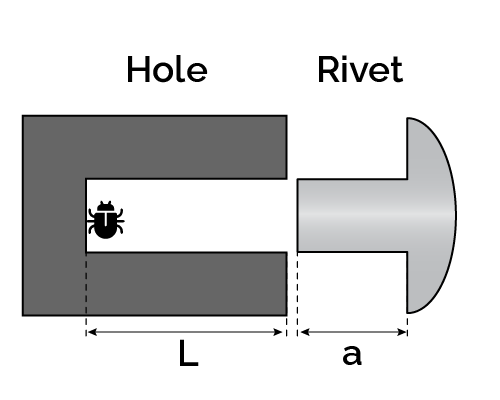
\includegraphics[width=0.5\linewidth]{Imágenes/bug-rivet-paradox_01_r2.png}
    \end{figure}    
\end{multicols}

\item Dos naves espaciales, cada una de \SI{100}{\m} de longitud (cuando se miden en reposo) viajan una hacia la otra con velocidades de $0.85c$ relativas a la Tierra.

    \begin{enumerate}
        \item ¿Qué longitud tiene cada nave medida por un observador desde la Tierra?

        \item ¿Qué velocidad tiene cada nave medida por un observador de la otra nave?

        \item ¿Qué longitud tiene cada nave medida por un observador de la otra nave?

        \item En el tiempo $t=0$ se ve desde la Tierra que las dos naves tienen sus extremos frontales en contacto, es decir, comienzan a cruzarse. ¿En qué momento se verán juntos desde la Tierra los extremos posteriores?
    \end{enumerate}

\end{enumerate}
\end{document}